\documentclass{article}
\usepackage{vs}
\begin{document}

\lecturetitle{Class 5 - Dimensionality Reduction}



\section{Singular Value Decomposition (SVD)}


\noindent We will see that any matrix $A \in \R^{m \times n}$ (w.l.o.g. $m \le n$) can be written as 
\begin{eqnarray}
A &=& \sum_{\ell=1}^{m} \sigma_{\ell} u_{\ell} v_{\ell}^{T}\\
&\forall \;\; \ell& \sigma_\ell \in \R,  \;\; \sigma_\ell \ge 0\\
&\forall \;\; \ell, \ell'&  \langle u_{\ell}, u_{\ell'} \rangle=  \langle v_{\ell}, v_{\ell'} \rangle = \delta(\ell,\ell')
\end{eqnarray}
%
To prove this consider the matrix $AA^{T} \in \R^{m\times m}$.
Set $u_\ell$ to be the $\ell$'th eigenvector of $AA^{T}$.
By definition we have that $AA^{T}u_\ell = \lambda_\ell u_\ell$.
Since $AA^{T}$ is positive semidefinite we have $\lambda_\ell \ge 0$.
Since $AA^{T}$ is symmetric we have that $\forall \;\; \ell, \ell' \;  \langle u_{\ell}, u_{\ell'} \rangle = \delta(\ell,\ell')$.
Set $\sigma_\ell = \sqrt{\lambda_\ell}$ and $v_\ell = \frac{1}{\sigma_\ell}A^{T}u_{\ell}$.
Now we can compute the following:
\[
\langle v_{\ell}, v_{\ell'} \rangle =  \frac{1}{\sigma^{2}_\ell}u_{\ell}^{T}AA^{T}u_{\ell'} =   \frac{1}{\sigma_{\ell}^{2}}\lambda_\ell  \langle u_{\ell}, u_{\ell'} \rangle = \delta(\ell,\ell')
\]
%
We are only left to show that $A = \sum_{\ell=1}^{m} \sigma_{\ell} u_{\ell} v_{\ell}^{T}$.
To do that consider the test vector $w = \sum_{i=1}^{m} \alpha_i u_i$.
\begin{eqnarray*}
|| w^{T}(A - \sum_{\ell=1}^{m} \sigma_{\ell} u_{\ell} v_{\ell}^{T})|| &=& || (\sum_{i=1}^{m}\alpha_i u^{T}_{i})(A - \sum_{\ell=1}^{m} \sigma_{\ell} u_{\ell} v_{\ell}^{T})|| \\
&=& || (\sum_{i=1}^{m}\alpha_{i} u^{T}_{i}A - \sum_{i=1}^{m}\sum_{\ell=1}^{m} \delta(i,\ell) \alpha_i \sigma_{\ell} v_{\ell}^{T}|| \\
&=& || (\sum_{i=1}^{m}\alpha_{i} \sigma_{i} v^{T}_{i} - \sum_{i=1}^{m} \alpha_i \sigma_{i} v_{i}^{T}|| = 0
\end{eqnarray*}
%
The vectors $u_\ell$ and $v_{\ell}$ are called the left and right singular vectors of $A$ and $\sigma_\ell$ are the singular vectors of $A$.
It is customary to order the singular values in descending order $\sigma_1 \ge \sigma_2, \ldots , \sigma_m \ge 0$.
Also, we will denote by $r$ the rank of $A$. 
Here is another very convenient way to write the fact that $A = \sum_{\ell=1}^{m} \sigma_{\ell} u_{\ell} v_{\ell}^{T}$
\begin{itemize}
\item Let $\Sigma \in \R^{r \times r}$ be a diagonal matrix whose entries are $\Sigma(i,i) = \sigma_i$ and $\sigma_1 \ge \sigma_2 \ge \ldots \ge \sigma_r$.
\item Let $U \in \R^{m \times r}$ be the matrix whose $i$'th column is the left singular vectors of $A$ corresponding to singular value $\sigma_i$.
\item Let $V \in \R^{n \times r}$ be the matrix whose $i$'th column is the right singular vectors of $A$ corresponding to singular value $\sigma_i$.
\end{itemize}
We have that $A = USV^T$ and that $U^{T}U = V^{T}V = I_r$. Note that the sum goes only up to $r$ which is the rank of $A$. Clearly, not summing up zero valued singular values does not change the sum.

\subsection*{Applications of the SVD}
\begin{enumerate}
\item Determining range, null space and rank (also numerical rank).
\item Matrix approximation.
\item Inverse and Pseudo-inverse: If $A=U \Sigma V^{T}$ and $\Sigma$
is full rank, then $A^{-1}=V \Sigma^{-1} U^{T}$. If $\Sigma$ is
singular, then its pseudo-inverse is given by $A^{\dagger}=V
\Sigma^{\dagger} U^{T}$, where $\Sigma^{\dagger}$ is formed by
replacing every nonzero entry by its reciprocal.
\item Least squares: If we need to solve $Ax=b$ in the least-squares
sense, then $x_{LS}=V \Sigma^{\dagger} U^{T} b$.
\item De-noising -- Small singular values typically correspond to
noise. Take the matrix whose columns are the signals, compute SVD,
zero small singular values, and reconstruct.
\item Compression -- We have signals as the columns of the matrix
$S$, that is, the $i$ signal is given by
\begin{equation*}
S_{i} = \sum_{i=1}^{r} \left ( \sigma_{j} v_{ij} \right ) u_{j}.
\end{equation*}
If some of the $\sigma_{i}$ are small, we can discard them with
small error, thus obtaining a compressed representation of each
signal. We have to keep the coefficients $\sigma_{j} v_{ij}$ for
each signal and the dictionary, that is, the vectors $u_{i}$ that
correspond to the retained coefficients.
\end{enumerate}

\noindent SVD and eigen-decomposition are related but there are quite a few differences between them.
\begin{enumerate}
\item Not every matrix has an eigen-decomposition (not even any
square matrix).  Any matrix (even rectangular) has an SVD.
\item In eigen-decomposition $A=X \Lambda X^{-1}$, that is, the
eigen-basis is not always orthogonal. The basis of singular vectors
is always orthogonal.
\item In SVD we have two singular-spaces (right and left).
\item Computing the SVD of a matrix is more numerically stable.
%\item Relation to condition number; the numerical problems with eigen-decomposition; multiplication by an orthogonal matrix is perfectly conditioned.
\end{enumerate}




\subsection*{Rank-k approximation in the spectral norm}
The following will claim that the best approximation to $A$ by a rank deficient 
matrix is obtained by the top singular values and vectors of $A$. More accurately:
\begin{fact}
Set
\begin{equation*}
A_{k} = \sum_{j=1}^{k} \sigma_{j} u_{j} v_{j}^{T}.
\end{equation*}
Then,
\begin{equation*}
\min_{\substack{B \in \mathbb{R}^{m \times n} \\
\operatorname{rank}(B) \leq k}} \norm{A-B}_{2} = \norm{A-A_{k}}_{2}
= \sigma_{k+1}.
\end{equation*}
\end{fact}


\begin{proof}
\begin{equation*}
\norm{A-A_{k}} = \norm{\sum_{j=1}^{r} \sigma_{j} u_{j} v_{j}^{T} - \sum_{j=1}^{k}
\sigma_{j} u_{j} v_{j}^{T}} = \norm{\sum_{j=k+1}^{r} \sigma_{j} u_{j}
v_{j}^{T}} = \sigma_{k+1} 
\end{equation*}
and thus $\sigma_{k+1}$ is the largest singular value of $A-A_{k}$.
Alternatively, look at $U^{T} A_{k} V =
\operatorname{diag}(\sigma_{1},\ldots,\sigma_{k},0,\ldots,0)$, which
means that $\operatorname{rank}(A_{k}) = k$, and that
\begin{equation*}
\norm{A-A_{k}}_{2} = \norm{U^{T} (A-A_{k}) V}_{2} =
\norm{\operatorname{diag}(0,\ldots,0,\sigma_{k+1},\ldots,\sigma_{r})}_{2}
= \sigma_{k+1}.
\end{equation*}

Let $B$ be an arbitrary matrix with $\operatorname{rank}(B_{k}) =
k$. Then, it has a null space of dimension $n-k$, that is,
\begin{equation*}
\operatorname{null}(B) = \operatorname{span}(w_{1},\ldots,w_{n-k}).
\end{equation*}
A dimension argument shows that
\begin{equation*}
\operatorname{span}(w_{1},\ldots,w_{n-k}) \cap
\operatorname{span}(v_{1},\ldots,v_{k+1}) \ne \{ 0 \}.
\end{equation*}
Let $w$ be a unit vector from the intersection. Since
\begin{equation*}
Aw = \sum_{j=1}^{k+1} \sigma_{j} (v_{j}^{T}w) u_{j},
\end{equation*}
we have
\begin{equation*}
\norm{A-B}_{2}^{2} \ge \norm{(A-B)w}_{2}^{2} = \norm{Aw}_{2}^{2} =
\sum_{j=1}^{k+1} \sigma_{j}^{2} \abs{v_{j}^{T}w}^{2} \ge
\sigma_{k+1}^{2} \sum_{j=1}^{k+1} \abs{v_{j}^{T}w}^{2} =
\sigma_{k+1}^{2},
\end{equation*}
since $w \in \operatorname{span}\{v_{1},\ldots,v_{n+1}\}$, and the
$v_{j}$ are orthogonal.
\end{proof}

\subsection*{Rank-k approximation in the Frobenius norm}

The same theorem holds with the Frobenius norm.
\begin{theorem} Set
\begin{equation*}
A_{k} = \sum_{j=1}^{k} \sigma_{j} u_{j} v_{j}^{T}.
\end{equation*}
Then,
\begin{equation*}
\min_{\substack{B \in \mathbb{R}^{m \times n} \\
\operatorname{rank}(B) \leq k}} \norm{A-B}_{F} = \norm{A-A_{k}}_{F}
= \sqrt{\sum_{i=k+1}^{m} \sigma_{i}^{2}}.
\end{equation*}
\end{theorem}
\begin{proof}
Suppose $A=U \Sigma V^{T}$. Then
\begin{equation*}
\min_{\operatorname{rank}(B) \leq k} \norm{A-B}^{2}_{F} =
\min_{\operatorname{rank}(B) \leq k} \norm{U \Sigma V^{T} - UU^{T} B
VV^{T}}^{2}_{F} = \min_{\operatorname{rank}(B) \leq k} \norm{\Sigma
- U^{T} B V}^{2}_{F}.
\end{equation*}
Now,
\begin{equation*}
\norm{\Sigma - U^{T} B V}^{2}_{F} = \sum_{i=1}^{n} \left (
\Sigma_{ii} - \left (U^{T}B V)_{ii} \right ) \right )^{2} +
\text{off-diagonal terms}.
\end{equation*}
If $B$ is the best approximation matrix and $U^{T}B V$ is not
diagonal, then write $U^{T}B V=D+O$, where $D$ is diagonal and $O$
contains the off-diagonal elements. Then the matrix $B = U D V^{T}$
is a better approximation, which is a contradiction.

Thus, $U^{T}B V$ must be diagonal. Hence,
\begin{equation*}
\norm{\Sigma - D}^{2}_{F} = \sum_{i=1}^{n} \left (\sigma_{i} - d_{i}
\right )^{2} = \sum_{i=1}^{k} \left (\sigma_{i} - d_{i} \right )^{2}
+ \sum_{i=k+1}^{n} \sigma_{i}^{2},
\end{equation*}
and this is minimal when $d_{i}=\sigma_{i}$, $i=1,\ldots,k$. The
best approximating matrix is $A_{k} = U D V^{T}$, and the
approximation error is $\sqrt{\sum_{i=k+1}^{n} \sigma_{i}^{2}}$.
\end{proof}


\section{Linear regression in the least-squared loss}
In Linear regression we aim to find the best linear approximation 
to a set of observed data. For the $m$ data  points $\{x_1,\ldots,x_m\}$,  $x_i \in \R^n$,
each receiving the value $y_i$, we look for the weight vector $w$ that minimizes:
\[
\sum_{i=1}^{n} (x_{i}^{T}w - y_i)^2 = \norm{Aw - y}_{2}^{2}
\]
Where $A$ is a matrix that holds the data points as rows $A_i = x^{T}_{i}$.

\begin{proposition}
The vector $w$ that minimizes $\norm{Aw - y}_{2}^{2}$ is $w = A^{\dagger}y = V\Sigma^{\dagger}U^{T}y$
for $A = U\Sigma V^T$ and $\Sigma^{\dagger}_{ii} = 1/\Sigma_{ii}$ if $\Sigma_{ii} > 0$ and $0$ else. 
\end{proposition}

Let us define $U_{\parallel}$ and $U_{\perp}$ as the parts of $U$ corresponding to positive and zero singular values of $A$ respectively. 
Also let $y_{\parallel} = 0$ and $y_{\perp}$ be two vectors such that $y = y_{\parallel}+y_{\perp}$ and 
$U_{\parallel}y_{\perp} = 0$ and $U_{\perp}y_{\parallel}=0$.

Since $y_{\parallel}$ and $y_{\perp}$ are orthogonal we have that  $\norm{Aw - y}_{2}^{2}
= \norm{Aw - y_{\parallel}-y_{\perp}}_{2}^{2} = \norm{Aw - y_{\parallel}}_{2}^{2} + \norm{y_{\perp}}_{2}^{2}$.
Now, since $y_{\parallel}$ is in the range of $A$ there is a solution $w$ for which $\norm{Aw - y_{\parallel}}_{2}^{2} = 0$.
Namely, $w = A^{\dagger}y = V\Sigma^{\dagger}U^{T}y$ for $A = U\Sigma V^{T}$. This is because $U\Sigma V^{T}V\Sigma^{\dagger}U^{T}y = y_{\parallel}$.
Moreover, we get that the minimal cost is exactly $ \norm{y_{\perp}}_{2}^{2}$ which is independent of $w$.


\section{PCA, Optimal squared loss dimension reduction}

Given a set of $n$ vectors $x_1,\ldots,x_n$ in $\R^{m}$. We look for a rank $k$ 
projection matrix $P \in \R^{m \times m}$ that minimizes:
\[
\sum_{i=1} ||Px_{i} - x_{i}||_{2}^{2}
\]
If we denote by $A$ the matrix whose $i$'th column is $x_i$ then this is equivalent to minimizing $||PA - A||_{F}^{2}$
Since the best possible rank $k$ approximation to the matrix $A$ is $A_{k} = \sum_{i=1}^{k}\sigma_{i}u_{i}v_{i}^{T}$ the best
possible solution would be a projection $P$ for which $PA = A_{k}$. This is achieved by $P = U_{k}U_{k}^{T}$ where $U_{k}$
is the matrix corresponding to the first $k$ left singular vectors of $A$. 

If we define $y_i = U_{k}^{T}x_{i}$ we see that the values of $y_i \in \R^{k}$ are optimally fitted to the set of points $x_i$ in the 
sense that they minimize:
\[
\min_{y_1,\ldots,y_n } \min_{\Psi \in \R^{k \times m}}\sum_{i=1} ||\Psi y_i - x_{i}||_{2}^{2}
\] 
The mapping of $x_i \rightarrow  U_{k}^{T}x_i = y_i $ thus reduces the dimension of any set of points  $x_1,\ldots,x_n$ in $\R^{m}$ to 
a set of points $y_1,\ldots,y_n$ in $\R^{k}$ optimally in the squared loss sense. This is commonly referred to as Principal Component Analysis (PCA).



\begin{center}
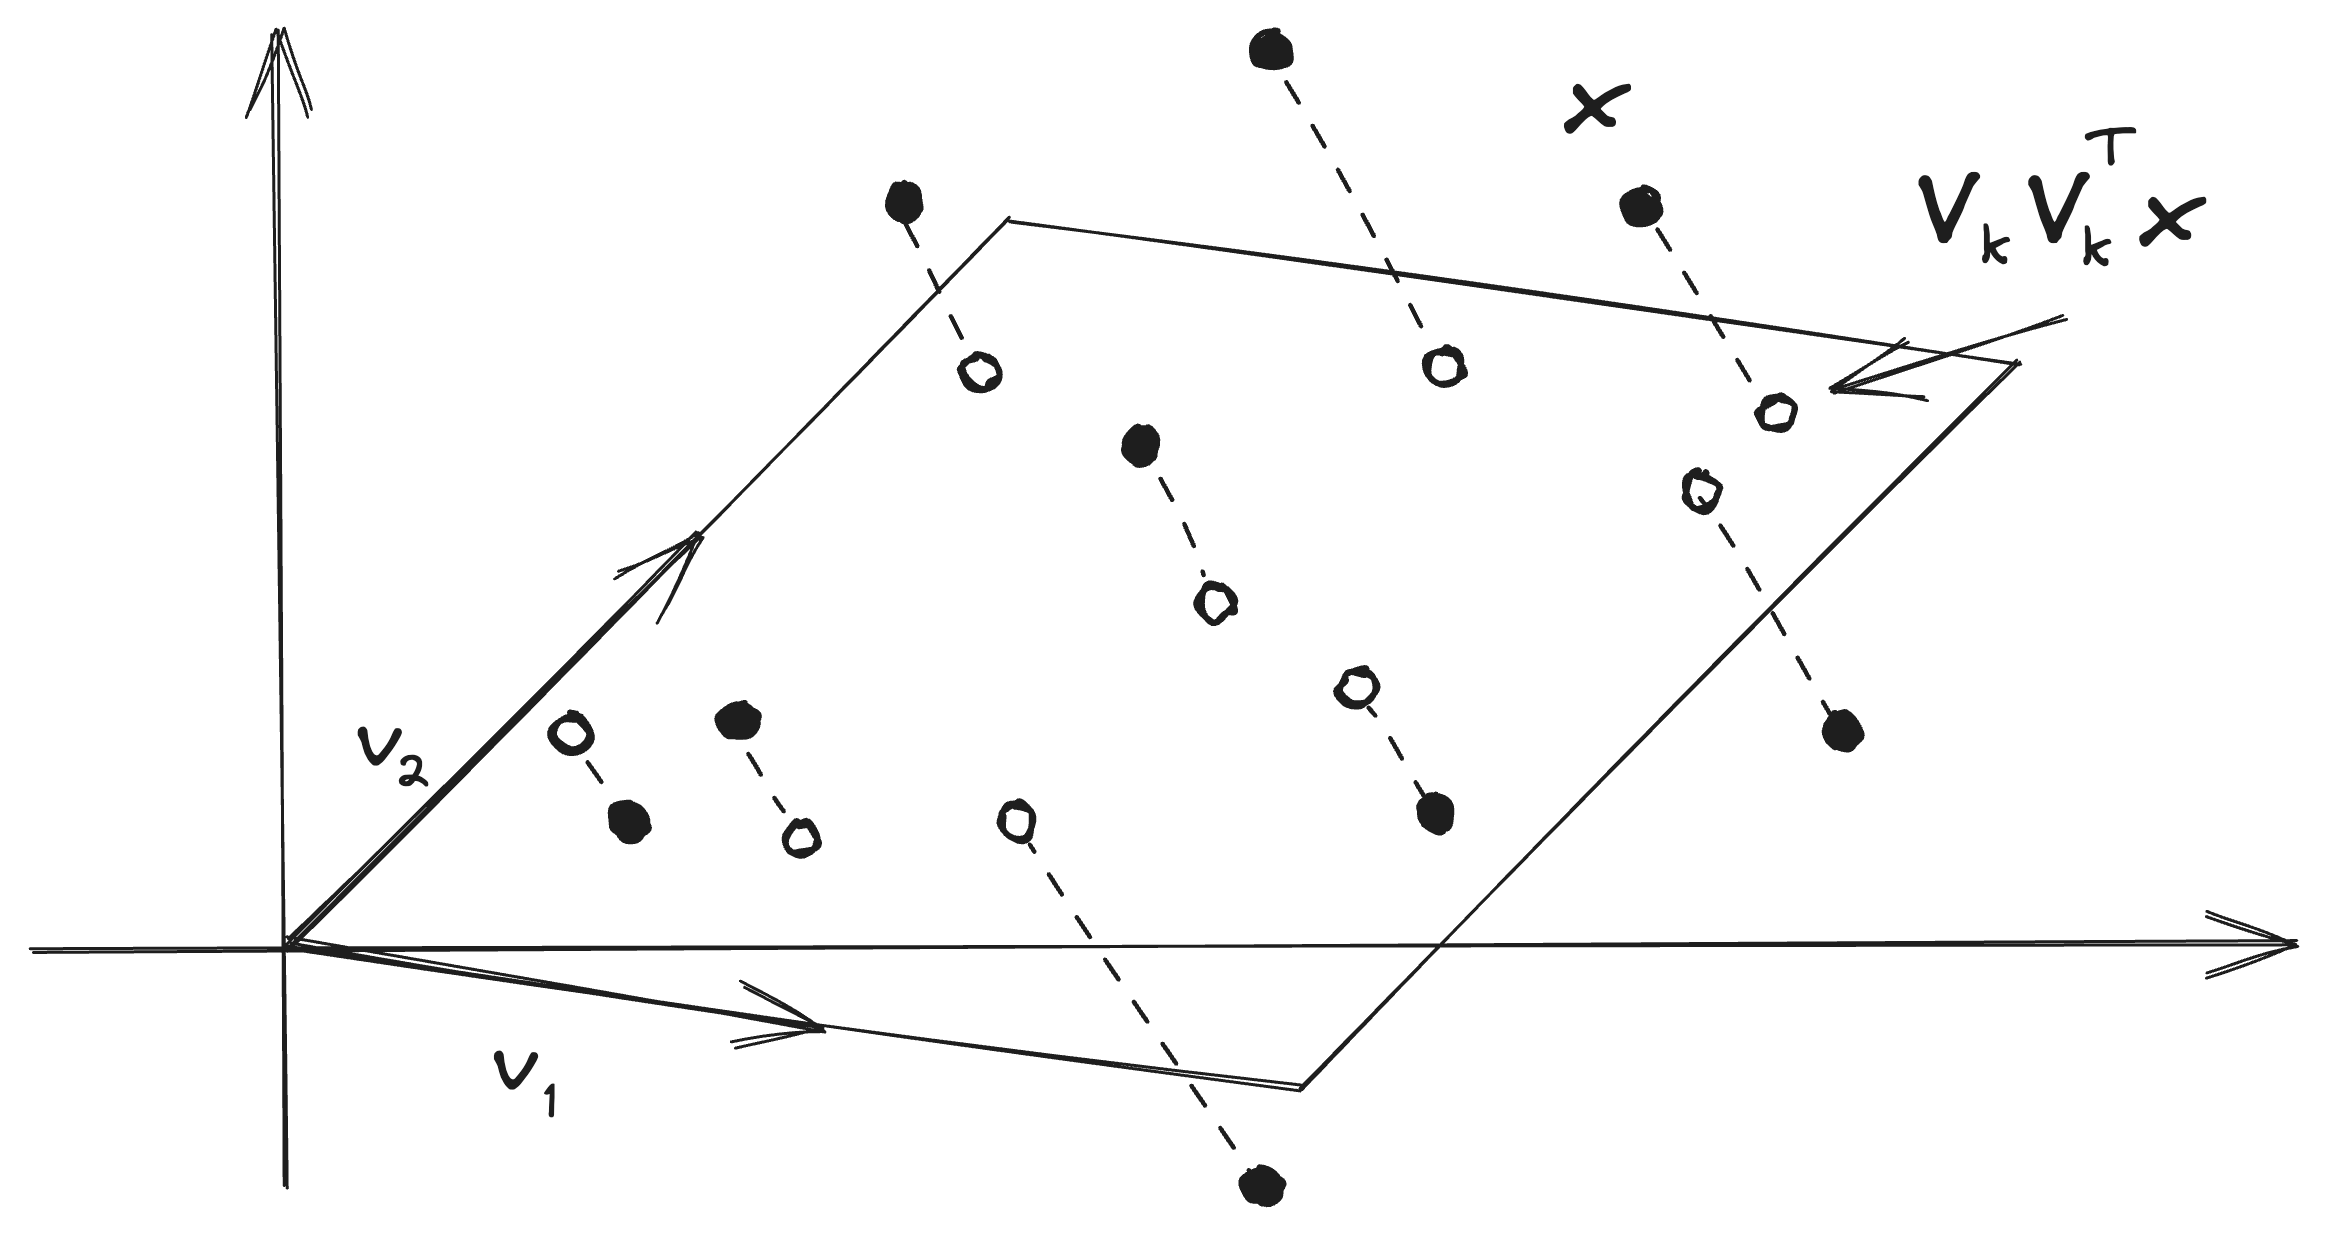
\includegraphics[width=0.6\textwidth]{images/pca.png}
\end{center}


\section{Closest orthogonal matrix}
The SVD also allows to find the orthogonal matrix that is closest to
a given matrix. Again, suppose that $A = U \Sigma V^{T}$ and $W$ is
an orthogonal matrix that minimizes $\norm{A-W}^{2}_{F}$ among all
orthogonal matrices. Now,
\begin{equation*}
\norm{U \Sigma V^{T} - W}_{F}^{2} = \norm{U \Sigma V^{T} - UU^{T} W
VV^{T}} = \norm{\Sigma - \tilde{W}},
\end{equation*}
where $\tilde{W}=U^{T} W V$ is another orthogonal matrix. We need to
find the orthogonal matrix $\tilde{W}$ that is closest to $\Sigma$.
Alternatively, we need to minimize $\norm{\tilde{W}^{T} \Sigma -
I}_{F}^{2}$.

If $U$ is orthogonal and $D$ is diagonal and positive, then
\begin{equation}\label{eq1}
\begin{aligned}
\operatorname{trace} (UD) &= \sum_{i,k} u_{ik} d_{ki} \leq \sum _{i}
\left ( \left ( \sum_{k} u_{ik}^{2} \right )^{1/2} \left ( \sum_{k}
d_{ik}^{2} \right )^{1/2} \right ) \\
&= \sum_{i} \left ( \sum_{k} d_{ki}^{2} \right )^{1/2} = \sum_{i}
\left ( d_{ii}^{2} \right )^{1/2} = \sum_{i} d_{ii} =
\operatorname{trace}(D).
\end{aligned}
\end{equation}
Now
\begin{align*}
\norm{\tilde{W}^{T} \Sigma - I}_{F}^{2} &= \operatorname{trace}
\left ( \left( \tilde{W}^{T} \Sigma - I \right ) \left(
\tilde{W}^{T} \Sigma - I \right )^{T} \right ) \\
&= \operatorname{trace} \left ( \left( \tilde{W}^{T} \Sigma   - I
\right
) \left( \Sigma \tilde{W}  - I \right ) \right ) \\
&= \operatorname{trace} \left ( \tilde{W}^{T} \Sigma^{2} \tilde{W}
\right ) - \operatorname{trace} \left ( \tilde{W}^{T} \Sigma \right
) - \operatorname{trace} \left ( \Sigma \tilde{W} \right ) + n \\
&= \operatorname{trace} \left ( \left ( \Sigma \tilde{W} \right
)^{T} \left ( \Sigma \tilde{W}  \right ) \right ) - 2
\operatorname{trace} \left (\Sigma \tilde{W} \right ) + n \\
&= \norm{\Sigma \tilde{W}}_{F}^{2} - 2 \operatorname{trace} \left
(\Sigma \tilde{W} \right ) + n \\
&= \norm{\Sigma }_{F}^{2} - 2 \operatorname{trace} \left (\Sigma
\tilde{W} \right ) + n.
\end{align*}
Thus, we need to maximize $\operatorname{trace} \left (\Sigma
\tilde{W} \right )$. But this is maximized by $ \tilde{W} = I$ by
\eqref{eq1}. Thus, the best approximating matrix is $W=UV^{T}$.





\section{Computing the SVD: The power method}

We give a simple algorithm for computing the Singular Value Decomposition of a matrix $A \in \R^{m \times n}$.
We start by computing the first singular value $\sigma_1$ and left and right singular vectors $u_1$ and $v_1$ of $A$,
for which $min_{i<j}\log(\sigma_i/\sigma_j) \ge \lambda$:
\begin{enumerate}
\item Generate $x_0$ such that $x_0(i) \sim \N(0,1)$.
\item $s \leftarrow  \log(4\log(2n/\delta)/\eps\delta)/2\lambda$ 
\item for $i$ in $[1,\ldots,s]$:
\item \tab $x_i \leftarrow A^{T}Ax_{i-1}$
\item $v_1 \leftarrow x_i/\norm{x_i}$  
\item $\sigma_1 \leftarrow \norm{Av_1}$
\item $u_1 \leftarrow Av_1/\sigma_1$ 
\item return $(\sigma_1,u_1,v_1)$ 
\end{enumerate}
Let us prove the correctness of this algorithm.
First, write each vector $x_i$ as a linear combination of the right singular values of $A$ i.e. $x_i = \sum_{j} \alpha^{i}_{j}v_j$. 
From the fact that $v_j$ are the eigenvectors of $A^{T}A$ corresponding to eigenvalues $\sigma^{2}_j$ 
we get that $\alpha^{i}_{j}= \alpha^{i-1}_{j}\sigma^{2}_{j}$.
Thus, $\alpha^{s}_{j} = \alpha^{0}_{j}\sigma^{2s}_{j}$. Looking at the ratio between the coefficients of $v_1$ and $v_i$ for $x_s$
we get that:
 \[
 \frac{|<x_s,v_1>|}{|<x_s,v_i>|} = \frac{|\alpha^{0}_{1}|}{|\alpha^{0}_{i}|}\left(\frac{\sigma_1}{\sigma_i}\right)^{2s}
\]
Demanding that the error in the estimation of $\sigma_1$ is less than $\eps$ gives the requirement on $s$.
\begin{eqnarray}
\frac{|\alpha^{0}_{1}|}{|\alpha^{0}_{i}|}\left(\frac{\sigma_1}{\sigma_i}\right)^{2s} &\ge& \frac{n}{\eps}\\
s &\ge& \frac{\log(n|\alpha^{0}_i|/\eps|\alpha^{0}|_1)}{2\log(\sigma_1/\sigma_i)}
\end{eqnarray}
From the two-stability of the Gaussian distribution we have that $\alpha^{0}_i \sim \N(0,1)$. 
Therefore, $\Pr[\alpha^{0}_i > t] \le e^{-t^2}$ which gives that with probability at least $1-\delta/2$ we have for
all $i$, $|\alpha^{0}_i | \le \sqrt{\log(2n/\delta)}$. Also, $\Pr[|\alpha^{0}_1 | \le \delta/4 ] \le \delta/2$ (this is because 
$\Pr[|z| < t] \le max_{r}\Psi_{z}(r)\cdot2t$ for any distribution and the normal distribution function at zero takes it maximal value which is less than $2$) 
Thus, with probability at least $1-\delta$ we have that for all $i$, $\frac{|\alpha^{0}_{1}|}{|\alpha^{0}_{i}|} \le \frac{\sqrt{\log(2n/\delta)}}{\delta/4}$.
Combining all of the above we get that it is sufficient to set $s = \log(4n\log(2n/\delta)/\eps\delta)/2\lambda = O(\log(n/\eps\delta)/\lambda)$
in order to get $\eps$ precision with probability at least $1-\delta$.

We now describe how to extend this to a full SVD of $A$. Since we have computed $(\sigma_1,u_1,v_1)$, we can repeat this
procedure for $A - \sigma_{1}u_{1}v_{1}^{T} = \sum_{i=2}^{n}{\sigma_{i}u_{i}v_{i}^{T}}$. The top singular value and vectors of which are $(\sigma_2,u_2,v_2)$.
Thus, computing the rank-k approximation of $A$ requires $O(mnks)  = O(mnk\log(n/\eps\delta))/\lambda)$ operations. 
This is because computing $A^{T}Ax$ requires $O(mn)$ operations and
for each of the first $k$ singular values and vectors this is performed $s$ times. 

The main problem with this algorithm is that its running time is heavily influenced by the value of $\lambda$.
This is, in fact, an artifact of the analysis rather than the algorithm. Next, we see a gap independent analysis.



\section{Gap independent analysis}
We show a short proof from \cite{liberty2016short} of a spectral gap independent property of simultaneous iterations. This follows the similar analyses \cite{RokhlinST09,HalkoMT2011,MuscoM15,WittenE15}. 

\begin{lemma} Let $A \in \R^{n \times m}$ be an arbitrary matrix and let $G \in \R^{m \times k}$ be a matrix of i.i.d.\ random Gaussian entries. 
Let $t = c\cdot \log(n/\eps)/\eps$ and $Z = \operatorname{span}((AA^T)^t A G)$ then
\[
||A - ZZ^TA|| \le (1+\eps)\sigma_{k+1}
\]
with high probability depending only on the universal constant $c$.
\end{lemma}
\begin{proof}
$||A - ZZ^TA|| = \max_{x :\|x\|=1}  \|x^T A\|$ such that $\|x^TZ\| = 0$.
We change variables $A = USV^T$ and $x = Uy$ and $G' = V^TG$.
Note that $G'$ is also a matrix of i.id.\ Gaussian entries because $V$ is orthogonal.
This reduces to 
$\max_{y:\|y\|=1}  \|y^TS\|$ such that $y^TS^{2t+1}G' = 0$.
We now break $y$, $S$, and $G'$ to two blocks each such that
\[
y =
\left(\begin{array}{c}
y_1 \\ \hline
y_2 \\
\end{array}\right)
%
\mbox{,\;\;}
%
S = \left(\begin{array}{c|c}
S_1 & 0 \\ \hline
0 & S_2 \\
\end{array}\right)
%
\mbox{,\;\;}
%
G' = \left(\begin{array}{c}
G'_1  \\ \hline
G'_2 \\
\end{array}\right)
\] 
and $y_1 \in \R^{k}$, $y_2 \in \R^{n-k}$, $S_1 \in \R^{k \times k}$, $S_2 \in \R^{(n-k) \times (n-k)}$, $G'_1 \in \R^{k \times k}$, and $G'_2 \in \R^{(n-k) \times k}$.
\begin{eqnarray*}
0 &=& \|y^T S^{2t+1} G'\| = \|y_1^T S^{2t+1}_1 G'_1+  y_2^T S^{2t+1}_2 G'_2\| \\
&\ge& \|y_1^T S^{2t+1}_1 G'_1\| -  \|y_2^T S^{2t+1}_2 G'_2\| \\
&\ge& \|y_1^T S^{2t+1}_1\|/\|G'^{-1}_1\| - \|y_2^T\| \cdot \|S^{2t+1}_2 \| \cdot  \|G'_2\| \\
&\ge& |y_1(i)| \sigma_{i}^{2t+1}/\|G'^{-1}_1\| - \sigma_{k+1}^{2t+1} \cdot  \|G'_2\| \ .
\end{eqnarray*}
\noindent This gives that $|y_1(i)| \le (\sigma_{k+1}/\sigma_i)^{2t+1}\|G'_2\| \|G'^{-1}_1\|$. Equipped with this inequality we bound the expression $\|y^TS\|$.
Let $k' \le k$ be such that $\sigma_{k'} \ge (1+\eps)\sigma_{k+1}$ and $\sigma_{k'+1} < (1+\eps)\sigma_{k+1}$.
\begin{eqnarray}
||A - ZZ^TA||^2 &=& \|y^TS\|^2 = \sum_{i=1}^{k'}y^2_i \sigma_i^2 + \sum_{i=k'+1}^{n}y^2_i \sigma_i^2 \\
&\le& \left( \|G'_2\|^2 \|G'^{-1}_1\|^2 \sum_{i=1}^{k'}(\sigma_{k+1}/\sigma_i)^{4t}  \sigma_{k+1}^2 \right) + (1+\eps)\sigma_{k+1}^2 \\
&\le& \left[ \|G'_2\|^2 \|G'^{-1}_1\|^2 k (1/(1+\eps))^{4t} + (1+\eps)\right]\sigma_{k+1}^2 \le (1+2\eps)\sigma_{k+1}^2
\end{eqnarray}
The last step is correct as long as $ \|G'_2\|^2 \|G'^{-1}_1\|^2 k (1/(1+\eps))^{4t} \le \eps \sigma^2_{k+1}$ which holds for $t \ge \log(\|G'_2\|^2 \|G'^{-1}_1\|^2 k/\eps) /4\log(1+\eps) = O(\log(n/\eps)/\eps)$. The last inequality uses the fact that $G'_1$ and $G'_2$ are random gaussian due to rotational invariance of the Gaussian distribution. This means that $\|G'_2\|^2 \|G'^{-1}_1\|^2 = O(\operatorname{poly}(n))$ with high probability \cite{Rudelson08}.
Finally, $||A - ZZ^TA|| \le \sqrt{1+2\eps}\cdot\sigma_{k+1} \le (1+\eps)\sigma_{k+1}$.
\end{proof}




\section{Random-projection}

We will give a simple proof of the following, rather amazing, fact. Every set of $n$ points 
in a Euclidian space (say in dimension $d$) can be embedded into the Euclidean space of 
dimension $k = O(\log(n)/\eps^2)$ such that all pairwise distances are preserved up distortion $1\pm \eps$.
We will prove the construction of \cite{DasGuptaGupta99} which is simpler than the one in \cite{JL84}.


We will argue that a certain distribution over the choice of a matrix $\R \in \R^{k \times d}$ gives that:
\begin{equation}
\label{e1}
\forall x \in \Sph^{d-1} \;\; \Pr\left[ \left| ||\frac{1}{\sqrt{k}}Rx|| - 1 \right| > \eps \right] \le \frac{1}{n^2} 
\end{equation}
Before we pick this distribution and show that Equation~\ref{e1} holds for it, let us first see
that this gives the opening statement. 

Consider a set of $n$ points $x_1,\ldots, x_n$ in Euclidean space $\R^d$. Embedding these points
into a lower dimension while preserving all distances between
them up to distortion $1\pm \eps$ means approximately preserving the norms of all 
${n \choose 2}$ vectors $x_i - x_j$. Assuming Equation~\ref{e1} holds and using the union 
bound, this property will fail to hold for at least one $x_i - x_j$ pair with probability at most ${n \choose 2}\frac{1}{n^2} \le 1/2$.
Which means that all ${n \choose 2}$ point distances are preserved up to distortion $\eps$ with probability at least $1/2$.


\section{Matrices with normally distributed independent entries}
We consider the distribution of matrices $R$ such that each $R(i,j)$ is drawn independently from  a
normal distribution with mean zero and variance $1$, $R(i,j) \sim \N(0,1)$. We show that for this
distribution Equation~\ref{e1} holds for some $k \in O(\log(n)/\eps^2)$.

First consider the random variable $z = \sum_{j=1}^{d}r(j)x(j)$ where $r(j) \sim \N(0,1)$. 
To understand how the variable $z$ distributes we recall the two-stability of the
normal distribution. Namely, if $z_3 = z_2 + z_1$ and 
$z_1 \sim \N(\mu_1,\sigma_{1})$ and $z_2 \sim \N(\mu_2,\sigma_{2})$ then, $$z_3 \sim \N(\mu_1 + \mu_2,\sqrt{\sigma^{2}_{1} + \sigma^{2}_{2}}).$$
In our case,  $r(i)x(i) \sim \N(0,x_{i})$ and therefore, $z = \sum_{i=1}^{d}r(i)x(i) \sim \N(0,\sqrt{\sum_{i=1}^{d}x^{2}_{i}}) \sim \N(0,1)$.
%
Now, note that each element in the vector $Rx$ distributes exactly like $z$.
Defining $k$ identical copies of $z$, $z_1,\ldots,z_k$,
We get that $||\frac{1}{\sqrt{k}}Rx||$ distributes exactly like $\sqrt{\frac{1}{k}\sum_{i=1}^{k} z^{2}_{i}}$.
Thus, proving Equation~\ref{e1} reduces to showing that:
\begin{equation}
\Pr\left[ \left| \sqrt{\frac{1}{k}\sum_{i=1}^{k} z^{2}_{i}} - 1 \right| > \eps \right] \le \frac{1}{n^2} 
\end{equation}
for a set of independent normal random variables $z_1,\ldots,z_k \sim \N(0,1)$.
It is sufficient to demanding that $\Pr[\sum_{i=1}^{k} z^{2}_{i} \ge k(1+\eps)^2]$ and $\Pr[\sum_{i=1}^{k} z^{2}_{i} \le k(1-\eps)^2]$ are both smaller than $1/2n^2$.
We start with bounding the probability that $\sum_{i=1}^{k} z^{2}_{i} \ge k(1+\eps)$ (this is okay because $k(1+\eps) < k(1+\eps)^2$).
\[
\Pr[\sum z^{2}_{i} \ge k(1+\eps)] = \Pr[e^{\lambda \sum z^{2}_{i}} \le e^{\lambda k (1+\eps)}] \le (\E[e^{\lambda z^2}])^k/e^{\lambda k (1+\eps)}
\]
Since $z \sim \N(0,1)$ we can compute $\E[e^{\lambda z^2}]$ exactly:
\[
\E [e^{\lambda z^{2}}] = \frac{1}{\sqrt{2\pi}}\int_{-\infty}^{\infty} e^{\lambda t^{2}} e^{-\frac{t^{2}}{2}} dt =\frac{1}{\sqrt{2\pi}}\int_{-\infty}^{\infty} e^{-\frac{(t\sqrt{1-2\lambda})^{2}}{2}}dt = e^{\frac{1}{2} \log(1-2\lambda)}
\]
The final step is by substituting $t' = t\sqrt{1-2\lambda}$ and recalling that $\frac{1}{\sqrt{2\pi}}\int_{-\infty}^{\infty} e^{-\frac{t'^{2}}{2}}dt' = 1$.
Finally, using the fact that $log(\frac{1}{1-2\lambda}) \le 2\lambda + 4\lambda^2$ for $\lambda \in [0,1/4]$ we have:
\[
\E [e^{\lambda z^{2}}] = \frac{1}{\sqrt{1-2\lambda}} = e^{\frac{1}{2} \log(\frac{1}{1-2\lambda})} \le e^{\lambda + 2\lambda^2}
\]
Substituting this into the equation above we have that:
\[
\Pr \le e^{k(\lambda  + 2\lambda^2) - k\lambda (1+\eps)} = e^{ 2k\lambda^2 - k\lambda\eps}  = e^{ - k\eps^2/8}  
\]
for $\lambda \leftarrow \eps/4$. Finally, our condition that 
\[
\Pr[\sum_{i=1}^{k} z^{2}_{i} \ge k(1+\eps)] \le e^{ - k\eps^2/8} \le 1/2n^2
\]
is achieved by $k = c\log(n)/\eps^2$.
Calculating for $\Pr[\sum_{i=1}^{k} z^{2}_{i} \le k(1-\eps)]$ in the same manner shows that $k = c\log(n)/\eps^2$ is also sufficient for this case.
This completes the proof.





\section{Fast Random Projections}
We discussed in class the fact that random projection matrices cannot be made sparse in general.
That is because projecting sparse vectors and preserving their norm requires the projecting matrix is almost fully dense see also \cite{JelaniH2012} and \cite{KaneN12}.

But, the question is, can we actively make sure that $x$ is not sparse? If so, can we achieve a sparse random projection for non sparse vectors?
These two questions received a positive answer in the seminal work by Ailon and Chazelle \cite{AilonCh06}.
The results of \cite{AilonCh06} were improved and simplified over the years. See \cite{AilonL11} for the latest result and an overview.

In this lesson we will produce a very simple algorithm based on the ideas in \cite{AilonCh06}.
This algorithm will require a target dimension of $O(\log^2(n)/\eps^2)$ instead of $O(\log(n)/\eps^2)$ but will be much simpler to prove.

\subsection{Fast vector $\ell_4$ norm reduction}
The goal of this subsection is to devise a linear mapping which preserves vector's $\ell_2$ norms but reduces their $\ell_4$ norms with high probability.
This will work to our advantage because, intuitively, vectors whose $\ell_4$ norm is small cannot be too sparse.
For this we will need to learn what Hadamard matrices are.

Hadamard matrices are commonly used in coding theory and are conceptually
close for Fourier matrices. We assume for convenience that $d$ is a power of $2$ (otherwise we can pad out vectors with zeros).
The Walsh Hadamard transform of a vector $x \in \R^{d}$ is the
result of the matrix-vector multiplication $Hx$ where $H$ is a $d
\times d$ matrix whose entries are $H(i,j) = \frac{1}{\sqrt{d}}(-1)^{\langle
i,j\rangle}$. Here ${\langle i,j\rangle}$ means the dot product over
$F_2$ of the bit representation of $i$ and $j$ as binary vectors of
length $\log(d)$.
Another way to view this is to define Hadamard Matrices recursively.
\begin{equation*} %
H_{1} = \frac{1}{\sqrt{2}}\left(
          \begin{array}{rr}
            1 & 1 \\
            1 & -1\\
          \end{array}
        \right)
,\;\;
        H_{d} = \frac{1}{\sqrt{2}}\left(
          \begin{array}{r:r}
            H_{d/2} & H_{d/2} \\ \hdashline
            H_{d/2} & -H_{d/2}\\
          \end{array}
        \right)
\end{equation*} %
Here are a few interesting (and easy to show) facts about Hadamard matrices.
\begin{enumerate}
\item $H_d$ is a unitary matrix $\|Hx\| = \|x\|$ for any vector $x\in \R^d$.
%\item $H_{d}(i,j) \in \{ \frac{1}{\sqrt{d}},- \frac{1}{\sqrt{d}}\}$
\item Computing $x \mapsto Hx$ requires $O(d\log(d))$ operations.
\end{enumerate}


We also define a diagonal matrix $D$ to be such that $D(i,i) \in \{1,-1\}$ uniformly.
Clearly, we have that $\|HDx\|_2 = \|x\|_2$ since both $H$ and $D$ are isotropies.
Let us now bound $\|HDx\|_\infty$.
$(HDx)(1) = \sum_{i=1}^{d}H(1,i)D(i,i) x_i = \sum_{i=1}^{d}\frac{x_i}{\sqrt{d}}s_i$ where $s_i \in \{-1,1\}$ uniformly.
To bound this we recap Hoeffding's inequality.
\begin{fact}[Hoeffding's inequality]
Let $X_1,\ldots,X_n$ be independent random variables s.t. $X_i \in [a_i,b_i]$.
Let $X = \sum_{i=1}^{n} X_i$.
\begin{equation}
\Pr[|X - \E[X]| \ge t] \le 2e^{-\frac{2 t^2}{\sum_{i=1}^{n} (b_i -a_i)^2}}
\end{equation}
\end{fact}
Invoking Hoeffding's inequality and then the union bound we get that if $\|HDx\|_\infty \le \sqrt{\frac{c \log(n)}{d}}$ for all points $x$.
Remark, for this we assumed $\log(d) = O(\log(n))$ otherwise we should have had $\log(nd)$ in the bound. 
The situation, however, that the dimension is super polynomial in the number of points is unlikely. 
Usually it is common to have $n > d$.

\begin{lemma}
Let $x \in \R^d$ by such that $\|x\|=1$. Then:
\[
\|HDx\|^4_4 = O(log(n)/d)
\]
with probability at least $1-1/\poly(n)$
\end{lemma}
\begin{proof}
Let us define $y = HDx$ and $z_i$ = $y_i^2$. 
From the above we have that $z_i \le \frac{c \log(n)}{d} = \eta$ with probability at least $1-1/\poly(n)$.
The quantity $\|HDx\|^4_4 = \|y\|_{4}^{4} = \sum_{i}z_i^2$ is a convex function of the $z$ variables which is defined over a polytop $z_i \in [0,1]$ and $\sum_{i} z_i = 1$ (this is because $\|y\|_2^2 = 1$).
This means that its maximal value is obtained on an extreme point of this polytope. 
In other words, the point $z_1,\ldots,z_{1/\eta} = \eta$ and $z_{1/\eta+1},\ldots,z_{d} = 0$ or $z = [\eta,\eta,\ldots,\eta,\eta,0,0,0,\ldots,0,0,0]$.
Computing the value of the function in this point gives $\sum_{i}z_i^2 \le (1/\eta)\cdot (\eta^2) = \eta$. Recalling the $\eta = \frac{c \log(n)}{d}$ completes the proof.  
\end{proof}

\subsection{Sampling from vectors with low $\ell_4$ norms}
Here we prove a very simple fact. For vectors whose $\ell_4$ is low, dimensionality reduction can be obtained by sampling.


Let $y$ be a vector such that $\|y\|_2 = 1$. Let $z$ be a sampled version of $y$ such that $z_i = y_i/\sqrt{p}$ with probability $p$ and $0$ else. 
This is akin to sampling, in expectation, $d\cdot p$ coordinates from $y$ (and scaling them up by $1/\sqrt{p}$).
Note the $\E[\|z\|^2] = \E[\|y\|^2] = 1$ moreover:
\[
\Pr[|\|z\|^2 - 1| > \eps] = \Pr[|\sum z_i^2 - 1| > \eps] = \Pr[|\sum b_i y_i^2/p - 1| > \eps]
\]
Where $b_i$ are independent random indicator variables taking the $b_i = 1$ with probability $p$ and $b_i = 0$ else.
To apply Chernoff's bound we must assert that $y_i^2/p \le 1$. Let's assume this for now and return to it later.
Applying Chernoff's bound we get
\[
\Pr[|\sum b_i y_i^2/p - 1| > \eps] \le e^{-\frac{c\eps^2}{\sigma^2}}
\]
where $\sigma^2 = \sum_{i} \E[(b_i y_i^2/p)^2] = \|y\|_{4}^{4}/p$.
Concluding that
\[
\Pr[|\|z\|^2 - 1| > \eps] \le e^{-\frac{cp\eps^2}{\|y\|_4^4}}
\]
This shows that the concentration of the sampling procedure really depends directly on the $\ell_4$ norm of the sampled vector.
If we plug in the bound on $\|y\|_4^4 = \|HDx\|_4^4$ from the previous section we get 
\[
\Pr[|\|z\|^2 - 1| > \eps] \le e^{-\frac{cp\eps d}{\log(n)}} \le \frac{1}{\poly(n)}
\]
For some $p \in O(\log^2(n)/d\eps^2)$. 

\subsection{Random Projection by Sampling}
Putting it all together we obtain the following.
\begin{lemma}
Define the following matrices
\begin{itemize}
\item $D$: A diagonal matrix such that $D_{i,i} \in \{+1,-1\}$ uniformly.
\item $H$: The $d\times d$ Walsh Hadamard Transform matrix.
\item $P$: A `sampling matrix' which contains each row of matrix $I_d\cdot \sqrt{p}$ with probability $p= c\log^2(n)/d\eps^2$.
\end{itemize}
Then, with at least constant probability the following holds.
\begin{enumerate}
\item The target dimension of the mapping is $k = c\log^2(n)/\eps^2$ (a factor $log(n)$ worse than optimal).
\item The mapping $x \mapsto PHDx$ is a $(1\pm\eps)$-distortion mapping for any set of $n$ points. 
That is, for any set $x_1,\ldots,x_n \in \R^d$ we have
\[
\|x_i -x_j\|(1-\eps) \le \|PHDx_i  - PHDx_j\| \le \|x_i -x_j\|(1+\eps)
\]
\item Storing $PHD$ requires at most $O(d + k\log(d))$ space.
\item Applying the mapping $x \mapsto PHDx$ requires at most $d\log(d)$ floating point operations.
\end{enumerate}
\end{lemma}


\bibliographystyle{plain}
\bibliography{vs}

\end{document}
%%%%%%%%
